%%%%%%%%%%%%%%%%%%%%%%%%%%%%%%%%%%%%%%%%%
% FRI Data Science_report LaTeX Template
% Version 1.0 (28/1/2020)
% 
% Jure Demšar (jure.demsar@fri.uni-lj.si)
%
% Based on MicromouseSymp article template by:
% Mathias Legrand (legrand.mathias@gmail.com) 
% With extensive modifications by:
% Antonio Valente (antonio.luis.valente@gmail.com)
%
% License:
% CC BY-NC-SA 3.0 (http://creativecommons.org/licenses/by-nc-sa/3.0/)
%
%%%%%%%%%%%%%%%%%%%%%%%%%%%%%%%%%%%%%%%%%


%----------------------------------------------------------------------------------------
%	PACKAGES AND OTHER DOCUMENT CONFIGURATIONS
%----------------------------------------------------------------------------------------
\documentclass[fleqn,moreauthors,10pt]{ds_report}
\usepackage[english]{babel}
\graphicspath{{fig/}}
\usepackage{svg}
\usepackage{subfig}
\usepackage{float}



%----------------------------------------------------------------------------------------
%	ARTICLE INFORMATION
%----------------------------------------------------------------------------------------

% Header
\JournalInfo{FRI Data Science Project Competition 2024}

% Interim or final report
\Archive{Final report} 
%\Archive{Final report} 

% Article title
\PaperTitle{Classifying Psychiatric Disorders} 

% Authors (student competitors) and their info
\Authors{Ahmet Çalış, Manfred Gonzalez-Hernandez, and Joaquín Figueira}

% Advisors
\affiliation{\textit{Advisors: Prof. Dr. Jure Demšar}}

% Keywords
\Keywords{Data Science, Psychiatry, fMRI, B-SNIP, GBC, FC, Network Analysis, ML, DS}
\newcommand{\keywordname}{Keywords}


%----------------------------------------------------------------------------------------
%	ABSTRACT
%----------------------------------------------------------------------------------------
\Abstract{

In recent times the need for a bioneurological basis to treat psychosis spectrum disorders has become apparent, as the clinical treatment of these disorders still relies on self-reported behavioral analysis of the patients which has proven to be inaccurate. In this work we use dimensionality reduced data from fMRI scans to predict the disorders of a set of 711 psychosis spectrum disorder patients and control group, with the ultimate goal of finding a small latent space of the fMRI data in which the different disorders and their symptoms are clearly distinguishable. To achieve this goal we combine approaches from traditional Machine Learning, Network Analysis and Dimensionality Reduction. The results suggest that it's possible to accurately differentiate a patient from the control group and map this distinction in a meaningful latent space, but predicting specific disorders within the patient group and symptomatic scales proved unsuccessful with the data and methodology applied.
}

%----------------------------------------------------------------------------------------

\begin{document}

% Makes all text pages the same height
\flushbottom 

% Print the title and abstract box
\maketitle 

% Removes page numbering from the first page
\thispagestyle{empty} 

%----------------------------------------------------------------------------------------
%	ARTICLE CONTENTS
%----------------------------------------------------------------------------------------

\section*{Introduction}

    Given the high levels of complexity of the human brain and its associated afflictions, diagnosing and treating psychiatric disorders is a notoriously challenging endeavor. This is specially true in the psychosis spectrum of disorders (PSD), where the literature shows that, due to its greater symptomatic variability, there is a pressing need for more complex and individualized patient care.

    One of the biggest impediments to this sort of treatment is the fact that traditional clinical approaches used to diagnose and treat these disorders relay on behavioral and self reported observations of the patients symptoms, such as the Positive and Negative Syndrome Scale (PANSS). Although a successful neural mapping across canonical schizofrenia (SZP) symptoms has been found in previous works \cite{Chen2020}, the field still lacks an accurate neural mapping for the full spectrum of pyschosis disorders. Finding such a mapping could be used to provide more accurate forms of treatments and diagnosis with a sound biomolecular basis.

    In this context, this project aims to bridge this behavioral and neurological gap by developing Machine Learning (ML) approaches to relate different patient fMRI scans with their corresponding PANSS scores, using data obtained by the Bipolar and Schizophrenia Network for Intermediate Phenotypes consortium (B-SNIP)\cite{Clementz2016}. The data consists of a set of PANSS scores and resting state fMRIs scans from patients diagnosed with schizophrenia (SZP), schizoaffective disorder (SADP) and bipolar disorder with psychosis (BPP), and a control group (CON). The ultimate objective of this work is to build a classifier that can accurately predict the specific disorder of a patient using their corresponding fMRI data, and use it to find a small latent space representation of the neural data that highly correlates to PSD symptoms.
    

\iffalse    
    Using this data we can also build Functional Connectivity representations between brain regions, which has been shown to find important patterns in brain activity \cite{Matkovič_2024, Wang2021-ts}. One of such representations are connectivity-based graphs convolutional networks (cGCN) architecture for fMRI analysis, allowing the extraction of spatial features from connectomic neighborhoods, showing effectiveness in individual identification and classification of ASD patients in \cite{Wang2021-ts}. The proposed architecture was applied to supervised classification experiments using rs-fMRI data from the Human Connectome Project, showcasing its performance in identifying subjects based on their rs-fMRI data.

        In addition to the patient and control groups PANSS scores, the data is composed of a set of time series of 3D-images for each patient of different regions of the brain, from which we obtain a set of correlation-based connectivity features by finding the correlations between regions across time. We used two of such connectivity feature extraction methods, which has been proposed as imaging markers for several psychiatric disorders \cite{Kraus2020-ut}. Using this data we implemented several Machine learning models to build a binary classifier of sick or healthy patients. Then we escalated the analysis to a multi-label classifier of the different diagnosis of the patients.
\fi


%------------------------------------------------

\section*{Methods}
\label{sec:methods}

\subsection*{Data preprocessing and dimensionality reduction}

An fMRI scan records the brain activity of a patient through blood oxygenation measurements. In these measurements the fMRI scanner intrinsically divides the brain into different regions (formally called voxels) according to a pre-defined spatial resolution, which tipycally results in a subdivision of the brain in around 90,000 voxels. The result is a time series of 3-D images of blood oxygenation levels for each voxel sampled with an approximate time resolution of 1.5 seconds during 20-30 minutes, which all combined amounts to very large data volumens for even a single patient.  

As the high dimensionality of this data representation would probably lead to high degrees of overfitting and excessively high runtimes, we used several dimensionality reduction techniques to make it more digestible. First, we merged voxels into regions of interest (ROIs), for which we used two parcellations: the Glasser parcellation which has 718 ROIs and the Cole-Anticevic parcellations whith 12 ROIs.

With this first reduction we obtained a time series of images with more compact resolutions. However, the data volume was still intractable due to the size of the time dimension of the series. To tackle this we used two other techniques for time dimensionality reduction: Functional Connectome (FC) and Global Brain Connectivity (GBC). The first approach, FC, measures the total correlation between each pair of ROIs across time. In other words, for a parcellation with $r$ ROIs, the data is reduced to a $\mathbb{R}^{r\times r}$ matrix. The second approach, GBC, computes the average correlation between one ROI and all the others across time, resulting in a $r$ dimensional vector. 

\subsection*{Traditional Machine Learning on GBC data}

%These are all the traditional machine learning algorithms we used over the tabular data
To tackle the problem of binary and multiclass disorder classification we first trained 12 different classifiers on the GBC data using the two parcellations previously described and all the features. We used 6 classifiers for binary health status classification and, 6 classifiers for multi-label disorder classification. 

To build these classifiers we used three learners: random forests, XGBoost and MLPs. As random forests are known to perform relatively well with little parameter and feature extraction procedures, we decided to use them as a general baseline. Since we're working in the medical domain, explainability is key, which is the reason why we decided to use XGBoost as our main classification model, as it provides both decent performance and explainability. Additionally, it can perform well in low sample environments. To test more complex feature interaction models, we decided to use Multi Layer Perceptrons (MLP). For training and evaluation we used a train-test split of the data with 20\% test size. We performed hyper-paramer tunning using the train split and for evaluation we computed the models' accuracy in the test split.

\subsection*{Feature Selection}

In the previous approach we found very poor performance in multiclass classification. A major issue we found with the data was the imbalance between the 718 features and the insufficient number of samples (638). This was our motivation to create a more involved feature selection process. Furthermore, in  implementing the previous approach we noted that performance dropped significantly with increased data compression. Consequently, we chose to work with 718 ROI Glasser parcellation data. 

First, we checked for constant and quasi constant values. Next, we performed feature correlations and removed 84 features using a correlation threshold of 0.8. 

Additionally, we used mutual information, ANOVA test and univariate model performances.

\begin{figure}[htbp]
    \centering
    \subfloat[]{
        \includesvg[width=0.45\linewidth]{fig/mutual_info.svg}
        \label{fig:mutual_information}
    }
    \subfloat[]{
        \includesvg[width=0.45\linewidth]{fig/anova.svg}
        \label{fig:anova_test}
    }
    \caption{Mutual information and ANOVA test results}
    \label{fig:joint_dist_grid}
\end{figure}
As seen in Figure (a) above, there was no clear cut off point for mutual information, so we removed features with mutual information below 0.5. Figure (b) shows results for ANOVA, it revealed more features that had no relationship with target value. We removed 129 features with help of these two processes.

For univariate model performance based feature selection, we trained decision trees for each feature and checked weather this features help to the model to perform better than random classifier. This process removed 7 features at the end.

All of the techniques we utilized so far helped us to remove 222 features in total. We decided to continue with step forward feature selection (SFS) from this point. All previous steps are prepared us for SFS since its computationaly expensive process. SFS identified 5 key features at the end. We used these 5 features to check model performances.

\subsection*{Network Analysis on FC data}
In the upcoming stage of our research, we develop a graph-based framework to enhance feature extraction methods and find approaches for multi-class classification accuracy. We employed an undirected graph for each patient from a functional connectivity matrix by adding edges based on a threshold determined by the standard deviation of the absolute values in the matrix. Initially, the function calculates the threshold as a specified multiple (given by the standard deviation (std) multiplier) of the standard deviation of the absolute connectivity values. Each node, corresponding to an entity in the matrix, is added to the graph. Then, for every pair of nodes, an edge is created if the absolute value of the connectivity strength between them exceeds the calculated threshold, excluding self-loops by ensuring the nodes are different. The weight of each edge corresponds to the original connectivity strength. This method results in a graph where only the strongest connections, those significantly above the average connectivity strength, are represented, highlighting the most prominent functional relationships within the network. 

By doing this we explored the features of two types of graphs, one graph with a higher standard deviation multiplier where the amount of edges between nodes will be considerably lower than the second graph that had a smaller standard deviation multiplier. This can be seen in tables \ref{tab:graph_statistics_2}. The inital idea is that these features could describe each patient's network and apply machine learning models over these features. But the performance was less than random guess.

Via these graphs we wanted to analyze the sub-graphs orbits using a different architecture. In this case we linked the nodes with the top K connectivity values of each of the regions, to be able to see how these sub-graphs expressed different information of the brain. To do so, we experimented with the Arithmetic Agreement similarity using the orbit counts using Orca \cite{orca} and then after applying the so called agreement similarity over all these graphs we built the figure \ref{fig:orca_blockmodel}  sorting the axes by the different groups or labels that each of the patient belongs to. The initial idea is that patients with the same label will highlight higher similarity near to the diagonal of the figure, but this did not happen.  

\begin{table}[h!]
\centering
\caption{\textbf{Summary of graph statistics for graphs with $STD=2$}. Notation:  $m$ = Number of Edges, $\langle K \rangle$ = Average Degree, Theoretical $\langle C \rangle$ = Theoretical Avg Clustering, $\langle C \rangle$ = Average Clustering, Theoretical $\langle PL \rangle$ = Theoretical Avg Path Length, $\langle PL \rangle$ = Average Path Length, CC = Size of Largest CC.}
\label{tab:graph_statistics_2}
\begin{tabular}{lrrrr}
\toprule
Statistic &       BPP &       CON &      SADP &      SCZP \\
\midrule
$m$                &  82137&  78250 &  78832 &  84185 \\
$\langle K \rangle$              &    228.79 &    217.97 &    219.59 &    234.50 \\
Theoretical $\langle C \rangle$  &      0.32 &      0.30 &      0.31 &      0.33 \\
$\langle C \rangle$              &      0.55 &      0.55 &      0.54 &      0.56 \\
Theoretical $\langle PL \rangle$ &      1.23 &      1.23 &      1.23 &      1.22 \\
$\langle PL \rangle$             &      1.69 &      1.71 &      1.70 &      1.68 \\
CC               &    717.83 &    717.88 &    717.84 &    717.89 \\
\bottomrule
\end{tabular}
\end{table}

\begin{table}[h!]
\centering
\caption{\textbf{Summary of graph statistics for graph with $STD=4.5$.} Same notation as in table \ref{tab:graph_statistics_2}.}
\label{tab:graph_statistics_4-5}
\begin{tabular}{lrrrr}
\toprule
label &      BPP &      CON &     SADP &     SCZP \\
\midrule
$m$                &  5083.51 &  1672.45 &  2622.66 &  8815.35 \\
$\langle K \rangle$              &    14.16 &     4.66 &     7.31 &    24.56 \\
Theoretical $\langle C \rangle$  &     0.02 &     0.01 &     0.01 &     0.03 \\
$\langle C \rangle$              &     0.11 &     0.09 &     0.09 &     0.12 \\
Theoretical $\langle PL \rangle$ &    12.08 &     9.37 &     8.18 &     6.69 \\
$\langle PL \rangle$             &     4.31 &     4.00 &     4.11 &     4.36 \\
CC               &   146.41 &   118.44 &   147.94 &   156.89 \\
\bottomrule
\end{tabular}
\end{table}

\begin{figure}[h!]
    \centering
    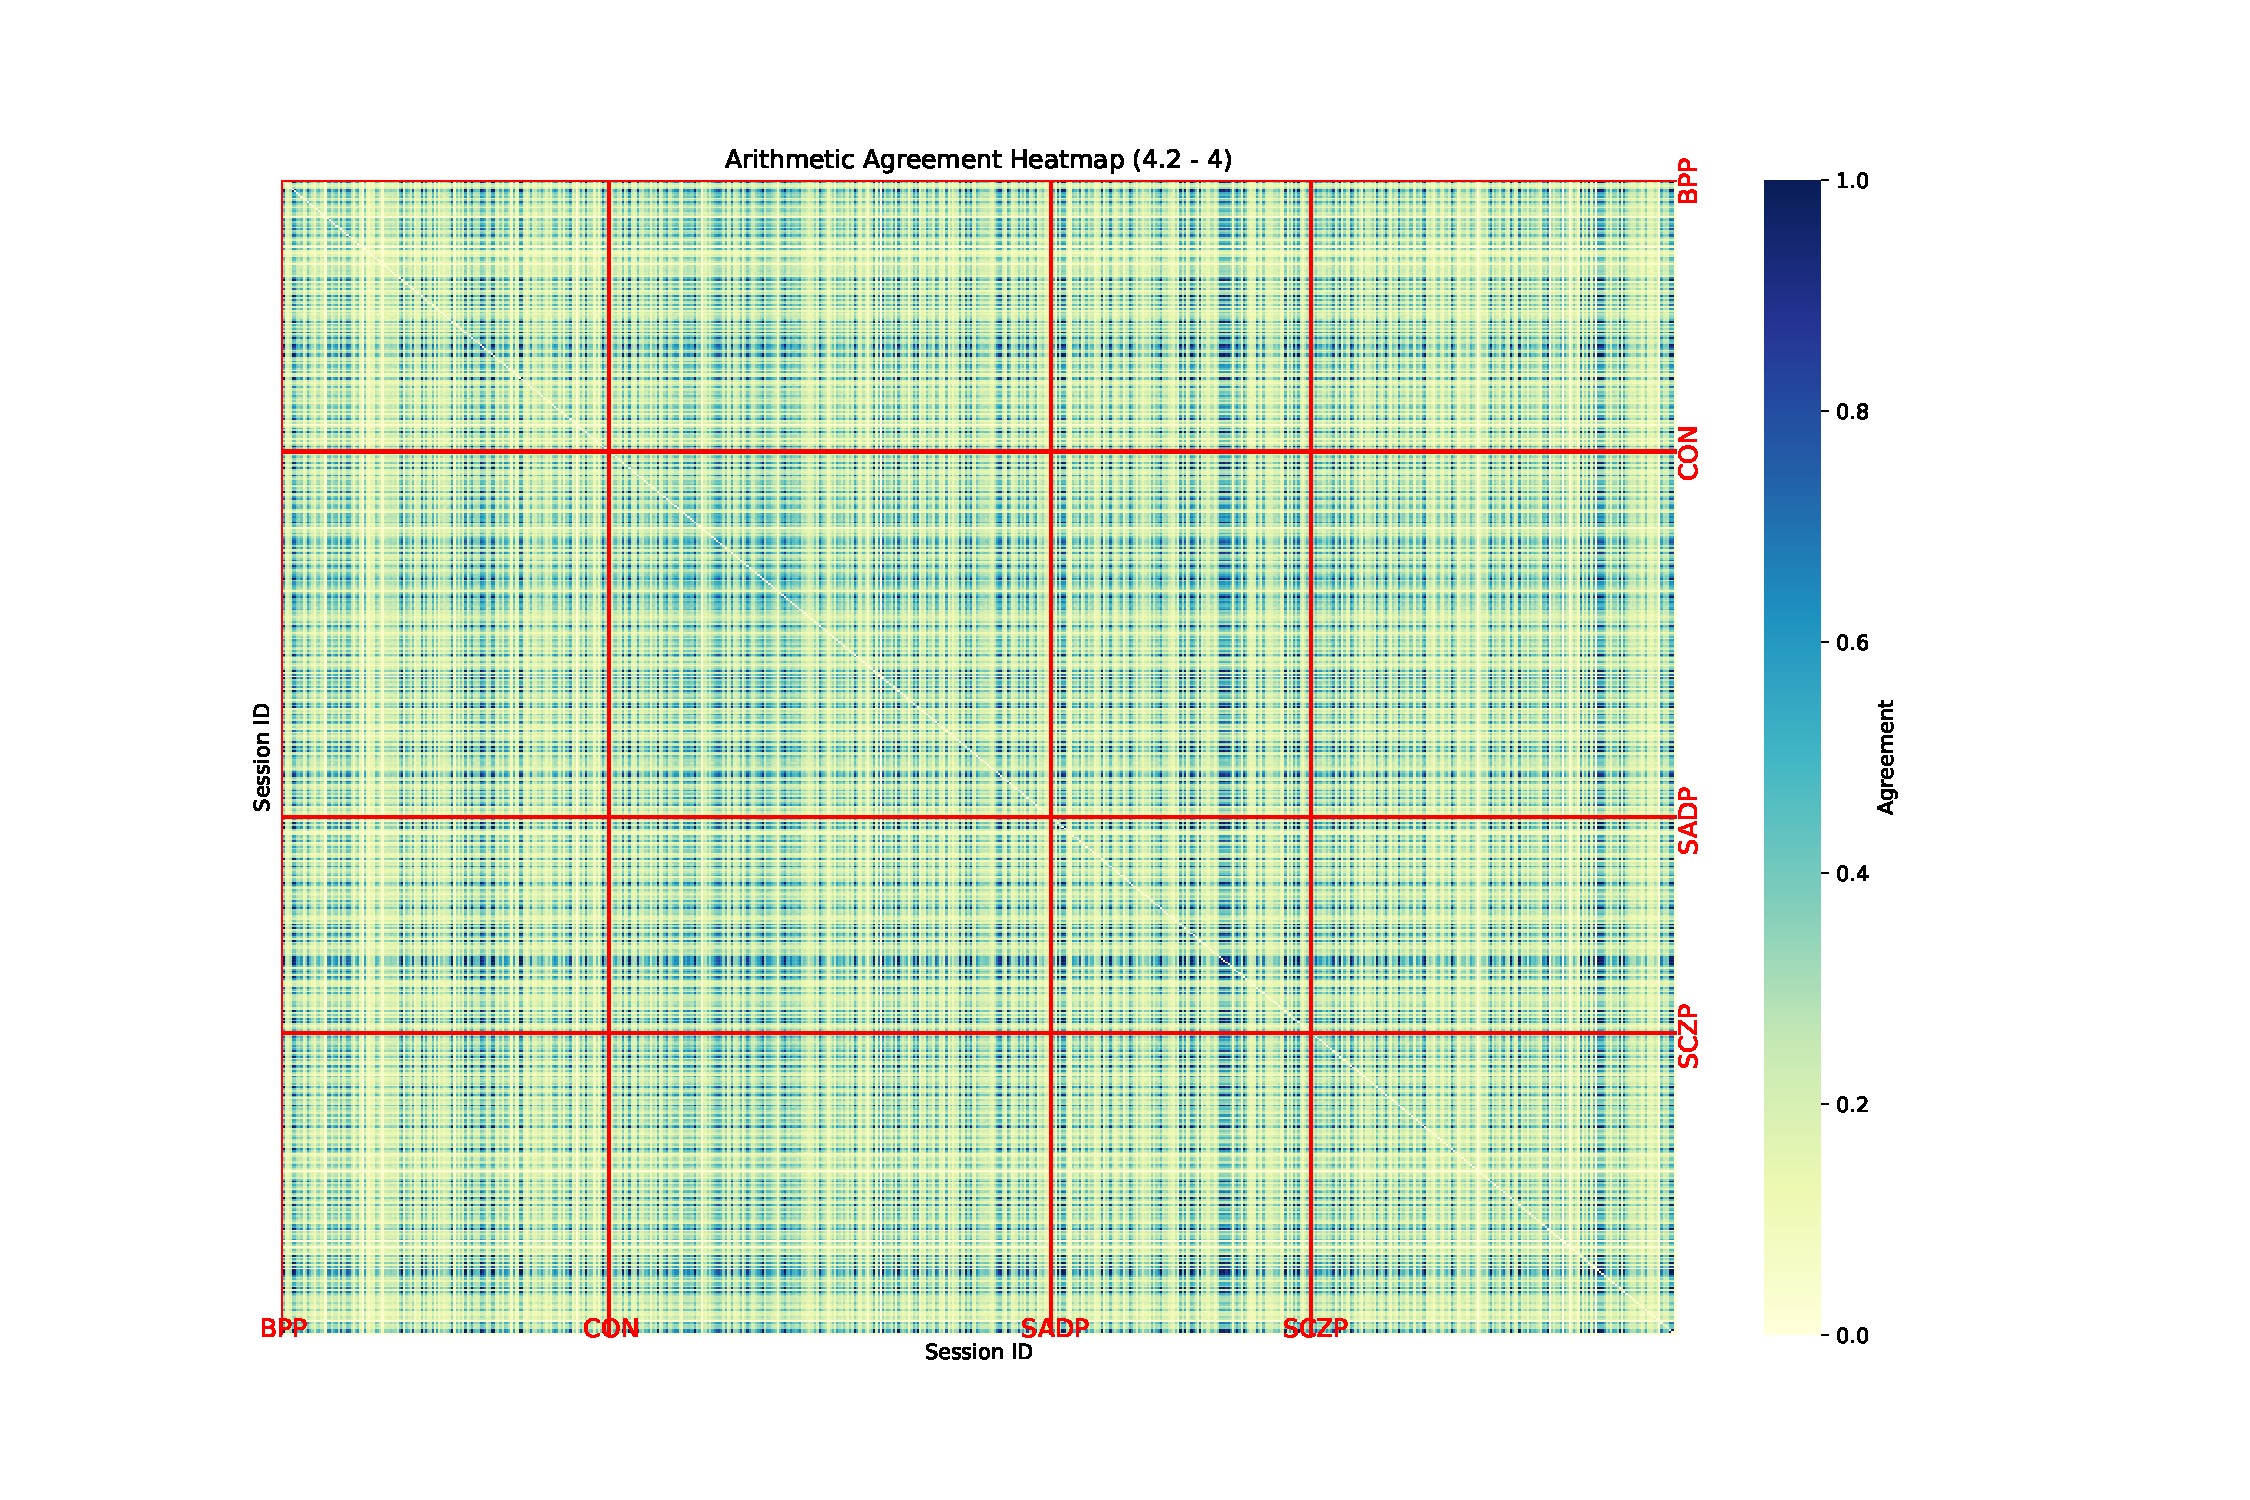
\includegraphics[width=\columnwidth]{fig/Arithmetic_Agreement_Heatmap_(4.2_-_4).pdf}
    \caption{Each pixel is the comparison of one session id FC graph with it's Arithmetic Agreement based on Orca orbits of 5 nodes. Each red line makes a boudary between session ids of different groups}
    \label{fig:orca_blockmodel}
\end{figure}


\subsection*{Latent Space representation}

As stated in the introduction of this paper, our ultimate goal was to find a mapping between PSD symptoms (encapsulated in the PANSS scores of the patients) and their neurological expression. To this end we developed a latent space representation technique to visually separate and cluster the different groups of patients. Ideally, a successful implementation of this approach should be able to correctly separate the different diagnosis into distinct clusters in a low dimensional space, allowing us to see possible similarities between them based on the distance and shapes of their clusters.

The technique we developed uses the 718 ROI parcellation GBC data to predict the PANSS scores of the patients using a Deep Neural Network (DNN) architecture with a central embedding layer. This layer has a small number of outputs that represent precisely the latent space of the GBC data. In a sense, we wanted to replicate an autoencoder architecture in which the input and output are (theoretically) correlated, but they're clearly distinct. 

The main hypothesis behind this implementation is that, if the diagnosis and associated symptoms are truly characterized by distinct brain patterns, then the network, while optimizing to reproduce the PANSS score, should be able to construct a latent or internal representation where disorders are clustered nicely. 

We tried several configurations of this base architecture using different number of hidden layers and different sizes of the embedding layer. In particular, we experimented with 2D and 3D embedding layers and one and two hidden layers in the encoder and decoder sections of the network. As we wanted to replicate the PANSS scores as precisely as possible we used Means Squared Error as loss function for the model.


\section*{Results} \label{results}

\subsection*{Traditional Machine Learning approach}

In this section we present the different results we obtained using a traditional machine learning approach using the GBC data. The results for the first approach using all the features and the 718 ROI Glasser parcellation are presented in table \ref{tab:glassier_classification} while the results after feature selection using only XGBoost are presented in tables \ref{tab:feature_selection_results}. Note that we omit the results for the Cole-Anticevic parcellation, as they were significantly lower even for binary classification (less than 0.7 accuracy). 

\begin{table}[h!]
\centering
\begin{tabular}{|l|l| c|c|c|}
\hline
\textbf{Metric} & \textbf{Type} & \textbf{XGBoost} & \textbf{Random Forest}& \textbf{MLP} \\ \hline
Accuracy (Tr) & Binary & 1.0 & 1.0 & 1.0 \\ \hline
Accuracy (Ts) & Binary & 0.984 & 0.977 & 0.98 \\ \hline
Accuracy (Tr) & Multi & 1.0 & 1.0 & 1.0 \\ \hline
Accuracy (Ts) & Multi & 0 & 0.586 & 0.55 \\ \hline
\end{tabular}
\caption{\textbf{Classification results before feature selection}. In the table \textit{Tr} stands for training and \textit{Ts} stands for Test. Furthermore, the type column indicates the task: \textit{Binary} for binary classification and \textit{Multi} for multiclass classification.}
\label{tab:glassier_classification}
\end{table}

\begin{table}[h!]
\centering
\begin{tabular}{|l|c|c|}
\hline
\textbf{Type} & \textbf{Accuracy (Tr)} & \textbf{Accuracy (Ts)}\\ \hline
Binary & 0.988 &  0.976 \\ \hline
Multi & 0.73 & 0.57\\ \hline
\end{tabular}
\caption{\textbf{Classification results after feature selection using XGBoost.} The notion is the same as in table \ref{tab:glassier_classification}.}
\label{tab:feature_selection_results}
\end{table}

It's clearly seen in the table above that feature selection didn't affect the performance on the test set and also helped to reduce overfitting, as performance in the training set decreased to a more realistic 0.73 and test set performance dropped only 1 percentage point. As the whole feature selection pipeline was based on multiclass labels, we also tested the models' performance for binary classification in order to validate that the 5 features selected are informative.

In conclusion, both multiclass and binary classification results indicate that only 5 features are sufficient for making reasonable predictions. We hypothesize that most features are uninformative due to excessive data compression during preprocessing. Furthermore, in terms of absolute performance, we can see that all models achieve very high accuracies for binary classification, even the baseline RF model. However, for multiclass classification we weren't able to improve accuracy from the baseline even after features selection.

\subsection*{Latent Space Representation}

In figure \ref{fig:latent_space_nn} we can visualize the results for the four architecture configurations we implemented. In it we can see the embeddings of the GBC data with 718 ROI labeled with their respective diagnosis. In all of the shallow representations we can see clear clusters separating patients from the control group. However, it seems the deep encoders compress the data too excessively by combining all the features multiple times. This results in very flat/uni-dimensional latent representations. Furthermore, none of the variations we tried were able to find a suitable representation where all the different groups are clearly differentiable.

\begin{figure}[h!]
    \centering
    \subfloat[2D Shallow Encoder]{
        \includesvg[width=0.45\linewidth]{fig/shallow_2d_encoder.svg}
    }
    \subfloat[3D Sahllow Encoder]{
        \includesvg[width=0.45\linewidth]{fig/shallow_3d_encoder.svg}
    } \\
    \subfloat[2D Deep Encoder]{
        \includesvg[width=0.45\linewidth]{fig/deep_2d_encoder.svg}
    }
    \subfloat[3D Deep Encoder]{
        \includesvg[width=0.45\linewidth]{fig/deep_3d_encoder.svg}
    }
    \caption{DNN latent space representation of the PANSS scores labeled with the patient disorders and control group.}
    \label{fig:latent_space_nn}
\end{figure}

As this results proved unsuccessful in segregating the different patient groups, we applied an additional dimensionality reduction technique known as t-SNE to see if we could improve them. In figure \ref{fig:tsne} we can see the results, where we can observe even less clearly defined clusters: although there seems to be an ordering distinction between patients and control groups, and an increased density in the region where the control group lies, the clusters are more dispersed in space. This serves as counterfactual evidence that there does seem to be some form of correlation between behavioral and neural data that which helps the DNN cluster the groups more efficiently.

\begin{figure}[h!]
    \centering
    \subfloat[t-SNE 2D latent space representation]{
        \includesvg[width=0.45\linewidth]{fig/tsne_2d_encoder.svg}
        \label{fig:joint_dist_stan_50}
    }
    \subfloat[t-SNE 3D latent space representation]{
        \includesvg[width=0.45\linewidth]{fig/tsne_3d_encoder.svg}
        \label{fig:joint_dist_stan_1000}
    }
    \caption{Latent space representation of the GBC 718 ROI parcellation using t-SNE labeled with the patient disorders and control group.}
    \label{fig:tsne}
\end{figure}


\section*{Discussion}
The results we obtained suggest that the problem of identifying the binary health status of a patient using biomarker data is solvable, as already suggested in the literature. We've proven this in multiple ways by building direct classifiers on the GBC data with high levels of precision and by sucessfuly encoding the data in a 2D and 3D latent space where control and patient groups are clearly discernible. We've also identified a relatively small number of regions of the Glasser parcelation where most of the differentiation between patient and control group seems to be originated. 

In relation to the Network Analysis of the FC data, we've determined that the specific combination of data and extensive analytical techniques we used is unable to tackle the problem of binary and multilabel classification of the different groups in the data. We hypothesize that the main probelm with our approach is the features extraction procedure, as extracting features manually from the graphs is challenging and it may require more advanced approaches such as graph embeddings or graph neural networks that are outside of the scope of this work.

Finally, all the approaches we experimented with for multilabel classification of the disorders proved unsucessful. We believe that the main reason for this is the large amounts of compression applied to the original data. Several of our results seem to support this conclussion. Firstly, we saw how important the ROI atlas in the classification power of our models with the drastic reduction in performance produced by the Cole-Anticevic Parcelation. It may be the case that other atlases with higher granularity may produce better results. Secondly, the low amount of ROIs (only 0.6\% of the all ROIs) that we identified were most correlated with predictive performance and the large correlation we saw between the features seem to suggest that GBC is too aggressive of a method to maintain relevant information from all the ROIs. 

\section*{Future Work}
Our results suggest that to solve the problem of multiclass classification of PSD new dimensionality reduction and representation techniques for fMRI data need to be developed. On the one hand, it'd be beneficial to develop different spatial reduction techniques and neural atlases with a focus on maintaining as much as possible the spatial variability of the data. We believe more fine grained atlases will be specially useful in this respect, as advances in Machine Learning in recent years make it feasible to train more complex algorithms such as DNN on this high dimensional data. 

Furthermore, we believe that to solve the task of multiclass classification of psychosis spectrum disorders temporal dimensionality reduction techniques such as GBC should be avoided. This is because such general approaches probably loose too much information in the compression of the feature interactions through time. Instead, we believe it'd be more effective to use sequence transformers on the raw ROIs activation time sequences, which can encode more complex feature interactions in the data through time. 

Finally, using more advanced network analysis techniques on the Functional Connectome data could provide better insights into the neurological study of PSD. In particular, it could help in finding improved graph representations of the data that could facilitate the use of ML techniques to find highly correlated ROIs in the brain to be targeted by specific medications.
%------------------------------------------------



%----------------------------------------------------------------------------------------
%	REFERENCE LIST
%----------------------------------------------------------------------------------------
\bibliographystyle{unsrt}
\bibliography{report}


\end{document}